\documentclass{article}
\usepackage[linesnumbered,lined,ruled,vlined]{algorithm2e}
\usepackage{graphicx}
\usepackage{xcolor}
\usepackage{listings}
\usepackage{float}
\usepackage{commath}

\definecolor{dkgreen}{rgb}{0,0.6,0}
\definecolor{gray}{rgb}{0.5,0.5,0.5}
\definecolor{mauve}{rgb}{0.58,0,0.82}
\definecolor{epurple}{rgb}{0.58,0,0.33}
\definecolor{eblue}{rgb}{0.31,0.45,1}

\lstdefinestyle{numbers} {numbers=left, stepnumber=1, numberstyle=\tiny, numbersep=10pt}
\lstdefinestyle{defs}{stringstyle=\color{eblue},keywordstyle=\color{epurple}}
\lstdefinestyle{MyJavaStyle} {language=Java,style=numbers,style=defs,frame=trBL,breaklines=true}
\lstdefinestyle{MyXMLStyle} {language=XML,style=numbers,style=defs,frame=trBL,breaklines=true}
\lstdefinestyle{MyPythonStyle} {language=Python,style=numbers,style=defs,frame=trBL,breaklines=true}

\graphicspath{ {img/} }

\title{Decision Tree on Hadoop}
\author{Md. Nazmul Alam (40016332), Newman (29469354)}

\renewcommand\lstlistingname{Code Snippet}
\renewcommand\lstlistlistingname{Code Snippets}

\begin{document}
\maketitle
\newpage
\tableofcontents
\listofalgorithms
\lstlistoflistings
\addtocontents{toc}{~\hfill\textbf{Page}\par}
\newpage
\section{Introduction}


Decision trees are commonly used in operations research, specifically in decision analysis, to help identify a strategy most likely to reach a goal, but are also a popular tool in machine learning\cite{wikidt}. However running decision tree on large dataset sequentially takes a lot of time. So, the natural evolution to optimize the sequential algorithm is to introduce parallel decision tree algorithm. Unlike sequential algorithm, parallel algorithm sometimes often tied to the parallel architecture on which it runs. Again, parallel architectures are not easily exposed or available to the algorithm itself. Hadoop implements MapReduce paradigm on commodity hardware in a distributed environment. The MapReduce paradigm reduces the complexity of programming and coordination of each node separately.
\BlankLine This report explores an algorithm for decision tree, which is implemented on hadoop, looks into the performance and covers some analysis of it. Following section describes the organization of this report.\BlankLine

Firstly the report covers about the MapReduce paradigm itself and how it works. This will give the reader a sense how an algorithm, intended to be implemented on a MapReduce environment, should be approached.

Next section will cover a simplified overview of the hadoop architecture and how to set up a two node cluster.

Next two sections will cover MapReduce version of word counting and matrix multiplication algorithms to enable the reader to visualize how an algorithm works in the MapReduce paradigm.

In the next section the report focuses on the main problem, decision tree. The report goes through the problem statement, current state of art and tries to give an overview of the problem. Then the report will look into the algorithm and how it works. Finally it provides the algorithms and code snippets along with the results for empirical studies of the algorithm in future.
In the closing sections, we will briefly go over possible future works and then draw the conclusion.

\section{Map Reduce}
Map reduce paradigm was first published in 2004 by Google in a white paper \cite{mrgoogle}. The idea behind it was to distribute a large set of data to multiple workers, whom will work in parallel. After their work, all the output are gathered and then another round of operation is performed to generate the final output. This kind of idea generally seems to be divide and conquer. Where large set of data is broken down and passed to initial workers. The operation performed by the initial worker is called map function, and trivially the workers are termed mapper. All the node executes the same mapper on a subset of the dataset and generate intermediate output. Then the output is grouped and passed to another set of worker. The operation performed by these worker are called reduce function, and the workers are termed reducer. The overall view can be understood from figure \ref{fig:mrp} \cite{c452017}. So, from a high-level MapReduce paradigm has 3 steps -
\begin{itemize}
\item Map
\item Combine/Shuffle
\item Reduce
\end{itemize}
\begin{figure}[h]
	\centering
	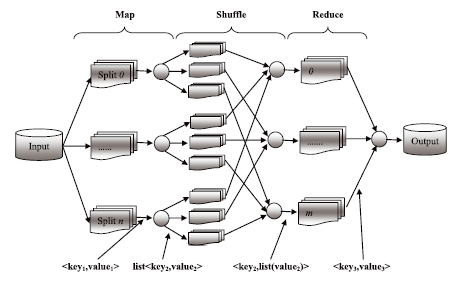
\includegraphics[width=\textwidth]{mr-hadoop-overview}
	\caption{Map Reduce Paradigm}
	\label{fig:mrp}
\end{figure}
To be highly distributed, there is no state kept between mapper or reducer. Hence MapReduce model was designed to works only with {key, value} pair data. So, in a typical MapReduce program, it takes in input data as {key, value} pair, perform map function to produce intermediate results containing a new {key, value} pairs, group the results from each mapper into {key, list{values}} and passes this new input to the reducer. Once the reducer performs the reduce operation a new {key, value} pair will be generated as output. Generally, a programmer is concerned with the implementation of the map and reduce function and let the default shuffle/combine operation to take place. However, generally, implementation of this paradigm also supports different Combine/Shuffle operation for complex requirements.

In the next section, this report provides a brief overview of the architecture of an open-source implementation of the MapReduce paradigm named Apache Hadoop.

\section{Hadoop Architecture}
\subsection {Overview}
Hadoop is an open-source implementation of the MapReduce paradigm. It is written in java. It generally supports any map/reduce implementation which runs on JVM (e,g java, scala), however, it can also support other language implementation via streaming API (e,g Python). From a very high level, the main components of Hadoop are -
\begin{itemize}
\item HDFS
\item Task Manager
\item Job Tracker
\item Name node
\item Data Node
\end{itemize}

The overall architecture is shown in figure \ref{fig:hadoop-arch} \cite{hadoopibm}.

\begin{figure}[h]
	\centering
	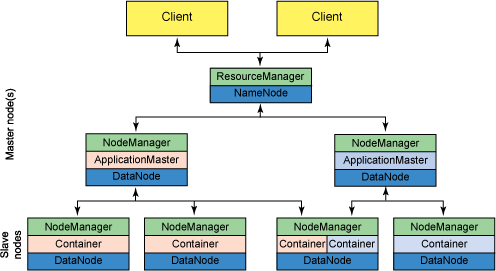
\includegraphics[width=\textwidth]{hadoop-arch}
	\caption{Hadoop Architecture}
	\label{fig:hadoop-arch}
\end{figure}

\subsection {Basic Architecture}

HDFS is the Hadoop Distributed File System, which performs the data replication on each of Datanode. So, any input or output written to HDFS by one node is available to any other node within that cluster. This abstracts the distributed programming complexities and lets the programmer focus on the actual algorithm.

\begin{figure}[h]
	\centering
	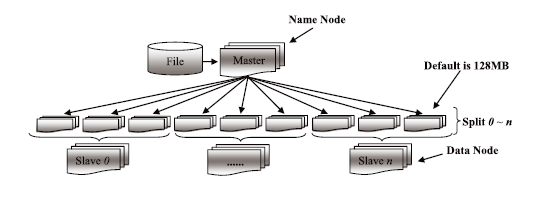
\includegraphics[width=\textwidth]{hadoop-hdfs}
	\caption{Map Reduce Paradigm}
	\label{fig:hdfs}
\end{figure}

Task Manager in the Hadoop framework is responsible for distributing the MapReduce application to the appropriate data node. More generally speaking its main task is to distribute the MapReduce task in each of the nodes and track its status.

Job Tracker generally runs in data node. The main functionality of it to run the assigned MapReduce task in the node and report back it’s status to Task manager.

Name node component defines the master node within the cluster. So, in the whole cluster, there will be a single name node.

Data node component defines the slave nodes within the cluster. Each processing node will have a component as a data node.

A very high-level relationship between this component is shown in figure \ref{fig:hdfs} \cite{c452017}.

\subsection{Setting Up Hadoop Cluster}
This section provides a high-level instruction on how to set up a Hadoop cluster on a Linux system. At the time of writing this report, the stable version of apache Hadoop was 2.7.3 \cite{hadoopap}.

Hadoop binary distributions are pretty much self-contained. The only dependencies Hadoop have are Java SDK and SSH-server. So, in Linux system one should install Java SDK (OpenJDK), ssh-server (e,g- OpenSSH-server) and ssh-client (generally preinstalled). After downloading the binary distribution, it should be extracted and placed in the desired location (e,g /usr/local/hadoop). It is not required but recommended to create a user account (e,g - hduser) to sandbox the access of Hadoop. In next section, it is provided how to setup a single node Hadoop. Once the individual single node is setup, a simple configuration will easily link them to make a two node setup.

\subsubsection {Single Node Setup}
The following instruction should be completed to enable single node Hadoop setup on a system -
\begin{itemize}
\item Generate ssh public/private key pair. Install the key on hduser account to enable auto login without any password.
\item Add HADOOP\_DIR, JAVA\_HOME in the environment variable
\item Edit \$\{HADOOP\_DIR\}/etc/hadoop/core-site.xml and add the following -\BlankLine
\begin{lstlisting}[caption={Hadoop CoreSite Config},label={lst:coresite},style=MyXMLStyle]
<property>
  <name>fs.defaultFS</name>
  <value>hdfs://master:9000</value>
</property>
\end{lstlisting}
\BlankLine Here the value of ``master'' is the IP address of the master node.
\item Edit \$\{HADOOP\_DIR\}/etc/hadoop/hdfs-site.xml and add the following -\BlankLine
\begin{lstlisting}[caption={Hadoop HDFS Config},label={lst:hdfssite},style=MyXMLStyle]
<property>
 <name>dfs.replication</name>
 <value>2</value>
</property>
<property>
 <name>dfs.permission</name>
 <value>false</value>
</property>
<property>
 <name>dfs.namenode.name.dir</name>
 <value>/usr/local/hadoop/hadoop_dir/namenode</value>
</property>
<property>
 <name>dfs.datanode.data.dir</name>
 <value>/usr/local/hadoop/hadoop_dir/datanode</value>
</property>
\end{lstlisting}
\BlankLine The value for ``name.dir'' and ``data.dir'' are used for name node and data node respectively. So, it must be ensured that these directories exist.

\item Copy the \$\{HADOOP\_DIR\}/etc/hadoop/mapred-site.xml.template to \$\{HADOOP\_DIR\}/etc/hadoop/mapred-site.xml and add the following - \BlankLine
\begin{lstlisting}[caption={Hadoop MapRed Config},label={lst:mapredsite},style=MyXMLStyle]
<property>
 <name>mapreduce.framework.name</name>
 <value>yarn</value>
</property>
\end{lstlisting}
\item Format the namenode using hdfs tool provided in the hadoop distribution
\end{itemize}

At this point single node setup is complete, to start Hadoop issue ``start-dfs.sh’’ and ``start-yarn.sh’’ subsequently.

\subsubsection{Multi Node Setup}
The following instruction should be completed to enable multi-node Hadoop setup -
\begin{itemize}
\item Add master ssh-pubkey to the trusted ssh-keys in the slaves. This enables autologin without any password.
\item Make sure each node can be run in single node setup
\item Create a new file in the master node  \$\{HADOOP\_DIR\}/etc/hadoop/slaves and enter all the slave IPs (including master if it is also a datanode)
\end{itemize}

At this point multi-node setup is complete, to start Hadoop issue ``start-dfs.sh'' and ``start-yarn.sh'' on the master to enable the auto-start of every slave as a data node.

\section{Word count}
\subsection{Problem Overview}
Word count problem is an introductory problem in MapReduce paradigm. It is very easy to parallelize and gives a very clear overview how MapReduce works.
\BlankLine The Word count problem, as the name implies, counts the number of unique words in a file. our implementation is case sensitive. If the dataset is very large then the sequential algorithm will take a long time to do the counting.
To use a parallel algorithm for it in MapReduce, it is important to think about how the input \{key,value\} pair should be prepared. What the mapper should produce and how the reducer will consume this to calculate the final result.
To fit this problem to the MapReduce pattern we start by creating a map function that can take the dataset and create a \{key,value\} pair.
This can be done by taking each word in a dataset and using that word as the key and the value as 1.

 For example the sentence "A This is a a word". Would map to
 \BlankLine \{"A", 1 \}, \{"This", 1 \}, \{"is", 1 \}, \{"a", 1 \}, \{"a", 1 \}, \{"word", 1 \}, \BlankLine The reduce part of the problem would take the \{key, value\} pairs and generate -
\BlankLine \{"A", 1 \}, \{"This", 1 \}, \{"is", 1 \}, \{"a", 2 \}, \{"word", 1 \}
\BlankLine In the section below the report defines the algorithm in psuedo code and one possible implementation in Python.
\subsection{Algorithm}
For mapper, the algorithm \ref{algo:wcmap} emits the word and count 1. In the reducer, the algorithm \ref{algo:wcred} emits the word and sum of the count.
\BlankLine
\IncMargin{1em}
\begin{algorithm}
\DontPrintSemicolon
\SetKwInOut{Input}{input}\SetKwInOut{Output}{output}
\SetKwFunction{emit}{emit}
\Input{(row\_id, text\_split)}
\Output{(word, 1)}
\BlankLine
\ForEach {$word\in text\_split$}{
\emit(word, 1)
}
\caption{Word Count Mapper\label{algo:wcmap}}
\end{algorithm}
\DecMargin{1em}

\IncMargin{1em}
\begin{algorithm}
\DontPrintSemicolon
\SetKwInOut{Input}{input}\SetKwInOut{Output}{output}
\SetKwFunction{emit}{emit}
\Input{(word, list(count))}
\Output{(word, sum)}
\BlankLine
$sum\leftarrow $0\;
\ForEach {$count\in list(count)$}{
	$sum\leftarrow $sum $+$ $count$
}
\emit(word, sum)\;
\caption{Word Count Reducer\label{algo:wcred}}
\end{algorithm}
\DecMargin{1em}
\subsection{Code Snippet}
In the code snippet \ref{lst:wcmap}, it generates the intermediate \{key, value\} pair. And the reducer can be implemented as code snippet \ref{lst:wcred}.


\begin{lstlisting}[caption={Word count mapper code},label={lst:wcmap},style=MyPythonStyle]
	import sys

	for line in sys.stdin:
		keys = line.strip().split()
		for key in keys:
	        	value = 1
	        	print( "%s\t%d" % (key, value) )

\end{lstlisting}

\BlankLine
\begin{lstlisting}[caption={Word count reducer code},label={lst:wcred},style=MyPythonStyle]

	import sys

	last_key = None
	running_total = 0
	count_map  = {}

	for input_line in sys.stdin:
		input_line = input_line.strip()
		this_key, value = input_line.split("\t", 1)
		value = int(value)
		count_map[this_key] = count_map.get(this_key,0) + value
		if last_key is None :
			last_key = this_key
		if last_key != this_key:
			print("%s\t%d" % (last_key, count_map.get(last_key,0)))
			last_key = this_key


	print("%s\t%d" % (last_key, count_map.get(last_key,0)))
\end{lstlisting}

\subsection{Analysis}
\BlankLine The sequential algorithm is $O(n)$ since the algorithm touch each word in order to count it and since the input has $N$ words, this is $O(n)$. For a parallel algorithm with $p$ processors and in each processor, it counts $\frac{n}{p}$ words. So this gives, $O(\frac{n}{p})$.


Parallel Algorithm Time, ${T_{p}}$ = $O(\frac{n}{p})$

Naive Sequential Algorithm, ${T_{s}}$ = $O(n)$

Number of processor, p = $p$

Speedup, ${S = T_{s}/T_{p}}$ = $\frac{O(n)}{O(\frac{n}{p})}$ = $O(p) = O(1)$ as $p << N$

Efficiency, ${E = S/p}$ = $\frac{O(p)}{p}$ = $O(1)$

\subsection{Results}
Word count implementation in Python took 3.4 seconds to count 50,000 words. It is apparent that disk I/O (communication time) is very high in streaming API compare to native (Java) application.
\section{Matrix multiplication}

\subsection{Problem Overview}
Matrix multiplication is a very common but highly practical operation. The problem of matrix multiplication is believed to be first formalized in the 19th century, however, proof does exist that it was being used even before that. There are many practical usages of large matrix multiplication, for example - simulation of galaxy systems, data analysis/mining, solving equations and much more.

Matrix multiplication can be defined as the multiplication of two matrix ${A_{P*Q},B_{Q*R}}$ to generate resultant matrix ${C_{P*R}}$ where ${C_{(i,j)}}$ is defined as
\begin{equation}
C_{(i,j)}\ =\ \sum_{k = 1}^{Q} A_{i, k} *  B_{k,j}
\end{equation}

In order to parallelize the matrix multiplication on a MapReduce paradigm, it is required to figure out -
\begin{itemize}
\item The input format
\item The intermediate output from mapper
\item How reducer will make the final result
\end{itemize}

From \(1\) it is evident that for to calculate the elements in a single row of the resultant matrix C, all of the values from the same row of A is required and all the values from the same column of B are required. In other words, to calculate the result for any ${C_{(i,j)}}$ the value ${A_{(i,0)} ... A_{(i,R)}}$ and ${B_{(0,j)} ... B_{(P,j)}}$ must be passed to a reducer. This simple analysis provides hints on the mapper\textsc{\char13}s output.

The map function needs to output for each value within a ${row_{x}}$ in A as ${I_{(x, 0)}, I_{(x, 1)} …  I_{(x,R)}}$ and for each value within a ${col_{y}}$ in B it needs to produce ${I_{(0, y)}, I_{(1, y)} …  I_{(P,y)}}$. All the ${I}$ values with same key will be  collected in the Shuffle/Combine step of map reduce. This ensures that a particular reducer will have all the values to compute 1 for a particular i,j.

The input of a particular matrix is given as ${(MatrixId,i,j,Value)}$ for each value of that matrix.

\subsection{Algorithm}
In the mapper algorithm, for each value of a matrix, if it is from $A$ is repeated up to the number of columns in matrix $B$. If the value is from $B$, it is repeated up to the number of rows in matrix $A$. The algorithm \ref{algo:mmmap} gives the pseudocode for the mapper function.\BlankLine
 
\IncMargin{1em}
\begin{algorithm}[H]
\DontPrintSemicolon
\SetKwInOut{Input}{input}\SetKwInOut{Output}{output}
\SetKwFunction{emit}{emit}
\SetKwFunction{GetColumnSize}{GetColumnSize}
\SetKwFunction{GetRowSize}{GetRowSize}
\Input{(row\_id, (matrix\_id, i, j, value))}
\Output{((a,b), (matrix\_id,j,value))}
\BlankLine
$Q\leftarrow \GetColumnSize($B)\;
$P\leftarrow \GetRowSize($A)\;
	\If{$matrix\_id\ equals\ $A}{
		\For {$k\leftarrow\ $0$\ \KwTo\ $Q}{
			\emit((i,k), (matrix\_id,j,value))
		}
	}
	\ElseIf{$matrix\_id\ equals\ $B}{
		\For {$k\leftarrow\ $0$\ \KwTo $P}{
			\emit((k,j), (matrix\_id,i,value))
		}
	}
\caption{Matrix Mul Mapper\label{algo:mmmap}}
\end{algorithm}
\DecMargin{1em}

\BlankLine In the reducer algorithm, all the required values from $A$ and $B$ are there. So, it needs to multiply the values from $A$ and $B$ which have the same indices. The algorithm \ref{algo:mmred} gives the pseudocode for the reducer function.\BlankLine

\IncMargin{1em}
\begin{algorithm}[H]
\DontPrintSemicolon
\SetKwInOut{Input}{input}\SetKwInOut{Output}{output}
\SetKwFunction{emit}{emit}
\SetKwFunction{GetColumnSize}{GetColumnSize}
\Input{(a,b), list(matrix\_id, i, value)}
\Output{((i,j), value)}
\BlankLine
$Q\leftarrow\ \GetColumnSize($A)\;
sort\ list\ into\ M\ or\ N\ based\ on\ i\;
$sum\leftarrow\ $0\;
\For{$K\leftarrow\ $0$\ \KwTo\ $Q} {
	$m_{ik}\leftarrow\ $0\;
	$n_{kj}\leftarrow\ $0\;
	\If{there\ is\ a\ value\ $K\ for\ $M} {
		$m_{ik}\leftarrow\ $M\big[K\big]
	}
	\If{there\ is\ a\ value\ $K\ for\ $N} {
		$n_{kj}\leftarrow\ $N\big[K\big]
	}
	$sum\leftarrow\ $sum $+$ ($m_{ik}$ $*$ $n_{kj}$)
}

\emit((i,k), sum)

\caption{Matrix Mul Reducer\label{algo:mmred}}
\end{algorithm}
\DecMargin{1em}

\subsection{Code Snippet}

The code snippet \ref{lst:mmmap} shows the java implements of the mapper.

\begin{lstlisting}[caption={Matrix multiplication mapper code snippet},label={lst:mmmap},style=MyJavaStyle]
protected void map(LongWritable key, Text value, Context context)
	throws IOException, InterruptedException {
	String [] values = value.toString().split(",");
	int lim_k = Integer.parseInt(context.getConfiguration().get("K"));
	int lim_m = Integer.parseInt(context.getConfiguration().get("M"));
	if (values[0].compareTo("M") == 0) {
		for(int k=0; k<lim_k; k++) {
			Text outputKey = new Text();
			Text outputValue = new Text();
			// key = i,k
			outputKey.set(values[1] + "," + k);
			// value = M,j,M(ij)
			outputValue.set("M," + values[2] + "," + values[3]);
			context.write(outputKey, outputValue);
		}
	} else {
		for(int k=0; k<lim_m; k++) {
			Text outputKey = new Text();
			Text outputValue = new Text();
			// key = k,j
			outputKey.set(k + "," + values[2]);
			// values = N,i,N(ij)
			outputValue.set("N," + values[1] + "," + values[3]);
			context.write(outputKey, outputValue);
		}
	}
}
\end{lstlisting}

Code snippet \ref{lst:mmred} shows the java implementation of the reducer.

\begin{lstlisting}[caption={Matrix multiplication reducer code snippet},label={lst:mmred},style=MyJavaStyle]
protected void reduce(Text arg0, Iterable<Text> arg1, Context arg2) throws java.io.IOException ,InterruptedException {
    String [] values;
    HashMap<Integer, Float> M = new HashMap<Integer, Float>();
    HashMap<Integer, Float> N = new HashMap<Integer, Float>();
    int lim_k = Integer.parseInt(arg2.getConfiguration().get("K"));
    for (Text val : arg1) {
        values = val.toString().split(",");
        if (values[0].compareTo("M") == 0) {
            M.put(Integer.parseInt(values[1]), Float.parseFloat(values[2]));
        } else {
            N.put(Integer.parseInt(values[1]), Float.parseFloat(values[2]));
        }
    }

    float result = 0.0f;
    float m_ik, n_kj;
    for(int k=0; k < lim_k; k++) {
        m_ik = M.containsKey(k) ? M.get(k) : 0.0f;
        n_kj = N.containsKey(k) ? N.get(k) : 0.0f;
        result += m_ik * n_kj;
    }

    arg2.write(null, new Text(arg0.toString() + "," + String.valueOf(result)));
}
\end{lstlisting}

\subsection{Analysis}
Let, A and B are the same $(N,N)$ matrix.
The algorithm described above has a mapper time complexity and a reducer time complexity.
The time complexity of mapper is ${O(N)}$. This is because, for each of the value, it has to produce N times of that value.
The time complexity of reducer is ${O(N)}$. This is because it iterates through N values of generated items from M and N and produces the final sum.
So, the overall time complexity of the parallel algorithm is ${O(N)}$\BlankLine

Parallel Algorithm Time, ${T_{p}}$ = ${O(N)}$

Naive Sequential Algorithm, ${T_{s}}$ = ${O(N^3)}$

Number of processor, p = ${N^2}$, as there are ${N^2}$ values for a particular matrix.

Speedup, ${S = T_{s}/T_{p}}$ = ${O(N^3)/O(N)}$ = ${O(N^2)}$

Efficiency, ${E = S/p}$ = ${O(N^2) / O(N^2)}$ = ${O(1)}$

\subsection{Results}
For the testing purpose, random values for large matrix was generated using a program. The randomness of the values is dependent upon the pseudo random function provided by the Java library. In a two node Hadoop cluster, the map-reduce application was executed.\BlankLine

In a $(50,50)$ A and B matrix the run time for MapReduce was approximately 2.5 seconds.

In a $(2000,2000)$ A and B matrix the run time for MapReduce was approximately 6.7 seconds.

It is apparent that in Hadoop implementation of MapReduce, the disk I/O is the major bottleneck for the performance \cite{c452017}.

\section{Decision tree}

\subsection{Problem Overview}
The focus of our paper is on decision trees, the decision tree can be used as a machine learning classifier \cite{quin1}.
The advantage of a decision tree is that it is a very simple algorithm to understand. The algorithm uses "purity" in order to recursively build the tree.
Two metrics are used to calculate the purity and what attributes to split on, namely entropy and information gain.
The disadvantage of a decision tree is that it is expnsive to build especially with a large dataset.
The problem that we will study is the implementation of C4.5 algorithm using the MapReduce framework.

\subsection{Literature Review}
We read several implementation of this algorithm using the MapReduce paradigm.
In \cite{c452017} the information gain ratio was calculated using a single MapReduce job.
While in \cite{c45cn} the information gain ratio was calculated from several MapReduce jobs.
In \cite{c45in} the information gain ratio is computed from the reduction of the map functions,
they write the information gain to a temporaray space which allows hadoop to access this data for the best attribute to split.
\cite{c45in} suffers from the fact that in highly distributed manner it might not be the case that the temporary file is avaible to other node,
 leading to wrong value for information gain ratio selection.
 Even if limiting the mapper to step forward will increase the parallel time and thus reducing the overall speedup and efficiency of the algorithm.
 \cite{c45cn} uses a very simple approach, using a pipeline of multiple map and reduce to build up the best attribute selection.
 Although it is simple, it incurs a lots of disk I/O in current hadoop implementation.
 However in recent hadoop implementation various optimization of disk I/O should reduce the issue.
 \cite{c452017} uses a more complicated mapper and reducer to select the best attribute.
  Compare to other two implementation it is much more optimized in term of number of rounds and disk I/O requirements.

\BlankLine
As the recursion part of the C4.5 to select the subsequent best attribute, recursion of the MapReduce algorithm is done to slowly build up the solution. In \cite{c45cn}, the proposed mechanism used a pipelined version of several MapReduce application, each performing a specific tasks. In \cite{c452017} and \cite{c45in} proposed method do not use pipelined version instead they rely on complex mapper and reducer.

\BlankLine
In the tree growing part for MapReduce C45, \cite{c452017}, \cite{c45cn} and \cite{c45in} uses some variant of MapReduce random forest grow algorithm.

\BlankLine
One major improvement was proposed in \cite{c45cn} by creating three special table to cache the calculation from previous step to the next step. According to their result, they claimed that with this modification they were able to outperform even with single node hadoop performance comparing with sequential algorithm. By using complex mapper and reducer, \cite{c452017} was able to reduce disk I/O overhead and thus increasing the overall algorithm performance. According to their claim, the proposed algorithm scales very well with commodity hardware.

\subsection{Methodology}

\subsection{Decision Tree Concept: Entropy}
Generally, entropy refers to disorder or uncertainty. In Information theory, entropy is the expected value (average) of the information contained in each message. 'Messages' can be modeled by any flow of information \cite{wikientropy}. In plain sentence entropy can be viewed as the chaos within a message. To understand why entropy is valuable in selecting an attribute over other, it is important to develop the intution on why a certain attribute is picked.

For an attribute ${X}$ such that it has 2 positive classifier and 2 negative classifier denoted by ${X_{2,2}}$, it is very difficult to make any kind of decision based on the attribute. Where considering another attribute ${Y}$ such that it has 3 positive classifier and 2 negative classifier denoted by ${Y_{2,2}}$, it is possible to say that it has a higher probably to correctly capture the positive classifier. Again an attribute ${Z}$ such that it has 2 positive and 3 negative classifier denoted by ${Z_{2,3}}$, it is possible to say that it has a higher probability to correctly capture the negative classifier. This probablitiy of an outcome helps to capture the entropy of an attribute. Figure \ref{fig:entropy} provides a very good view how entropy behaves. At probablity 0.5 the entropy is highest, making difficult to predict the outcome, where at probablity  0 and 1 the entropy is minimum, making very easy to predict the outcome.

\begin{figure}[H]
	\centering
	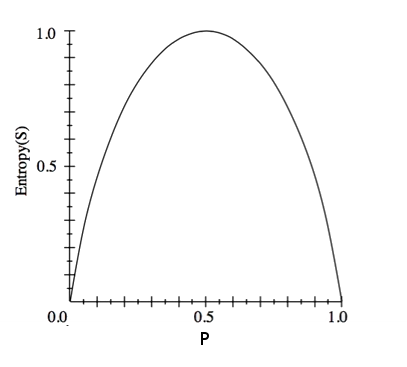
\includegraphics[width=200pt]{entropy}
	\caption{Relationship between entropy and probabliity}
	\label{fig:entropy}
\end{figure}

The equation for entropy is given by -
\begin{equation}
Entropy(a)\ = P(a)\ - \sum_{v \in values(C)}\log_{2}{P(a)}
\end{equation}
where C defines the set for classifier.

\subsection{Decision Tree Concept: Information Gain}
In decision tree, information gain means the mutual information carried by an attribute comparing to the classifier\cite{wikiinfogain}. In plain english, it is generally measure of ``information'' of a particular value of an attribute in contrast with entropy. For example, if an attribute holds ${X,Y,Z}$ values, each with different outcome. Then by contrasting each of them against the entropy of whole set, we can conclude which attribute should be the best node to pick.

The equation for information gain is given by -
\begin{equation}
IG(S, a)\ =\ Entropy(S)\ - \sum_{v \in values(a)}(\ \abs{x \in S\mid x_{a} = v}/\abs{T}\ ) * Entropy(x \in S\mid x_{a} = v)
\end{equation}

The goal is to pick the attribute with maximum information gain.

\subsection{Algorithm}

\IncMargin{1em}
\begin{algorithm}[H]
\DontPrintSemicolon
\SetKwInOut{Input}{input}\SetKwInOut{Output}{output}
\SetKwFunction{emit}{emit}
\Input{(row\_id, (${a_{j}}$), c)}
\Output{(${a_{j}}$,(row\_id, c))}
\BlankLine
\emit(${a_{j}}$,(row\_id, c))
\caption{Attribute Table Mapper\label{algo:atmap}} Sample reducer code in python.
\end{algorithm}
\DecMargin{1em}

\IncMargin{1em}
\begin{algorithm}[H]
\DontPrintSemicolon
\SetKwInOut{Input}{input}\SetKwInOut{Output}{output}
\SetKwFunction{emit}{emit}
\Input{(${a_{j}}$,list(row\_id, c))}
\Output{(${a_{j}}$,$(row\_id, c, count)$)}
\BlankLine
$count\leftarrow$ 0\;
\ForEach{$value \in$ list}{
	$count\leftarrow count + 1$\;
}
\emit(${a_{j}}$,(row\_id, c, count))
\caption{Attribute Table Reducer\label{algo:atred}}
\end{algorithm}
\DecMargin{1em}

\IncMargin{1em}
\begin{algorithm}[H]
\DontPrintSemicolon
\SetKwInOut{Input}{input}\SetKwInOut{Output}{output}
\SetKwFunction{emit}{emit}
\Input{(${a_{j}}$,$list(row\_id, c, count)$)}
\Output{(${a_{j}}$,$(row\_id, c, count, all)$)}
\BlankLine
$all\leftarrow$ 0\;
\ForEach{$value \in$ list}{
	$all\leftarrow all + 1$\;
}
\emit(${a_{j}}$,(row\_id, count, all))
\caption{Attribute Table Reducer 2\label{algo:atred_2}}
\end{algorithm}
\DecMargin{1em}

\IncMargin{1em}
\begin{algorithm}[H]
\DontPrintSemicolon
\SetKwInOut{Input}{input}\SetKwInOut{Output}{output}
\SetKwFunction{emit}{emit}
\SetKwFunction{Entropy}{Entropy}
\SetKwFunction{InfoGain}{InfoGain}
\SetKwFunction{SplitInfoGain}{SplitInfoGain}
\Input{(${a_{j}}$,$list(row\_id, c, count, all)$)}
\Output{(${a_{j}}$,$(InfoGain(a_{j}), SplitInfoGain(a_{j})))$}
\BlankLine
calc \Entropy(${a_{j}}$)\;
calc \InfoGain(${a_{j}}$) = ${(count/all) * Entropy(a_{j})}$\;
calc \SplitInfoGain(${a_{j}}$) = ${- (count/all) * \log_{2}{(count/all)}}$\;
\emit(${a_{j}}$,$(InfoGain(a_{j}), SplitInfoGain(a_{j}))$)
\caption{Attribute Selection Mapper\label{algo:atmap_2}}
\end{algorithm}
\DecMargin{1em}

\IncMargin{1em}
\begin{algorithm}[H]
\DontPrintSemicolon
\SetKwInOut{Input}{input}\SetKwInOut{Output}{output}
\SetKwFunction{emit}{emit}
\SetKwFunction{Entropy}{Entropy}
\SetKwFunction{InfoGain}{InfoGain}
\SetKwFunction{SplitInfoGain}{SplitInfoGain}
\Input{(${a_{j}}$,$(InfoGain(a_{j}), SplitInfoGain(a_{j})))$}
\Output{(${a_{j}}$,$(GainRatio(a_{j})$)}
\BlankLine
$gainRatio\leftarrow$ 0.0f\;
\ForEach{$value \in$ list}{
	$gainRatio\leftarrow gainRatio + (InfoGain(a_{j})/SplitInfoGain(a_{j}))$ \;
}
\emit(${a_{j}}$,$(GainRatio(a_{j})$)
\caption{Attribute Selection Reducer\label{algo:atred_3}}
\end{algorithm}
\DecMargin{1em}

% algorithm for best attribute selection -->

\IncMargin{1em}
\begin{algorithm}[H]
\DontPrintSemicolon
\SetKwInOut{Input}{input}\SetKwInOut{Output}{output}
\SetKwFunction{emit}{emit}
\SetKwFunction{Entropy}{Entropy}
\Input{(${a_{j}}$,$list(GainRatio(a_{j})$)}
\Output{(${a_{best}}$, count)}
\BlankLine
$a_{best}\leftarrow$\ empty\;
$maxGR\leftarrow 0$\;
\ForEach{$(a_{j}, GainRatio(a_{j})) \in$ list}{
	\If{$maxGR < GainRatio(a_{j})$}{
		$maxGR\leftarrow GainRatio(a_{j})$\;
		$a_{best}\leftarrow a_{j}$\;
	}
}
\emit(${a_{best}}$,$count$)
\caption{Attribute Selection Reducer 2\label{algo:atred_4}}
\end{algorithm}
\DecMargin{1em}

% end of algorithm

% algorithm for tree growing -->

\IncMargin{1em}
\begin{algorithm}[H]
\DontPrintSemicolon
\SetKwInOut{Input}{input}\SetKwInOut{Output}{output}
\SetKwFunction{emit}{emit}
\SetKwFunction{CreateSubNodeId}{CreateSubNodeId}
\SetKwFunction{hash}{hash}
\Input{(${a_{best}}$,$row\_id$)}
\Output{($row\_id$, (node\_id, subnode\_id))}
\BlankLine
$node\_id\leftarrow$\ \hash(${a_{best}}$)\;
\If{$node\_id$ already seen}{
	\emit($row\_id$, $node\_id$, $empty$)
}
\Else{
	$subnode\_id\leftarrow \CreateSubNodeId()$\;
	\emit($row\_id$, $node\_id$, $subnode\_id$)
}
\caption{Tree Grow Reducer\label{algo:atred_5}}
\end{algorithm}
\DecMargin{1em}

% end of algorithm

\subsection{Code Snippets}

% attribute selection mapper code

\begin{lstlisting}[caption={Attrib Table Mapper code snippet},label={lst:attrtblmap},style=MyJavaStyle]
protected void map(LongWritable key, Text value, Context context)
    throws IOException, InterruptedException {
    String [] values = value.toString().split(" ");
    String classifier = values[values.length - 1];
    System.out.println(value.toString() + ", Class: " + classifier);
    for(int i=0; i< values.length - 1; i++) {
        // write output as {key,value} => {attribute, (row_id, classifier)}
        Text outputValue = new Text();
        Text outputKey = new Text();
        outputKey.set(i+1 + " " + values[i]);
        outputValue.set(key.toString() + " " + classifier);
        context.write(outputKey, outputValue);
    }
}
\end{lstlisting}

% end of code snippet
% attribute selection reducer code

\begin{lstlisting}[caption={Attrib Table Reducer code snippet},label={lst:attrtblred},style=MyJavaStyle]
protected void reduce(Text arg0, Iterable<Text> arg1, Context arg2)
    throws IOException, InterruptedException {
    HashMap<String, HashMap<String, Integer>> classifierCount = new HashMap<String, HashMap<String,Integer>>();

    String key = arg0.toString();

    for (Text text : arg1) {
        String [] values = text.toString().split(" ");
        if (classifierCount.containsKey(key)) {
            if (classifierCount.get(key).containsKey(values[1])) {
                classifierCount.get(key).put(values[1],
                    classifierCount.get(key).get(values[1]) + 1);
            } else {
                    classifierCount.get(key).put(values[1], 1);
            }
        } else {
            HashMap<String, Integer> val = new HashMap<String, Integer>();
            val.put(values[1], 1);
            classifierCount.put(key, val);
        }
    }

    for (String keyAttribute : classifierCount.keySet()) {
        if (classifierCount.get(keyAttribute) != null) {
            for (String keyClass : classifierCount.get(keyAttribute).keySet()) {
                arg2.write(new Text(keyAttribute), new Text(keyClass + " " + classifierCount.get(keyAttribute).get(keyClass)));
            }
        }
    }
}
\end{lstlisting}

% end of code snippet

%code snippet for attrib selection reducer 2
\begin{lstlisting}[caption={Attrib Table Reducer 2 code snippet},label={lst:attrtblred2},style=MyJavaStyle]
protected void reduce(Text arg0, Iterable<Text> arg1,
    Context arg2)
    throws IOException, InterruptedException {
    long total = 0;
    LinkedList<String> set = new LinkedList<String>();

        for (Text text : arg1) {
        StringTokenizer tok = new StringTokenizer(text.toString());
        set.add(text.toString());
        String [] values = new String[tok.countTokens()];
        int i = 0;
        while(tok.hasMoreTokens()) {
            values[i++] = tok.nextToken().trim();
        }

        total += Long.parseLong(values[2]);
    }

    for (String text : set) {
        StringTokenizer tok = new StringTokenizer(text);
        String [] values = new String[tok.countTokens()];
        int i = 0;
            while(tok.hasMoreTokens()) {
                values[i++] = tok.nextToken().trim();
            }
        Text outputKey = new Text(arg0 + " " + values[0]);
        Text outputValue = new Text(values[1] + " " + values[2] + " " + String.valueOf(total));
        arg2.write(outputKey, outputValue);
    }
}
\end{lstlisting}
% end of code

% code for best attribute selection mapper
\begin{lstlisting}[caption={Attrib Selection Mapper code snippet},label={lst:attrselmap},style=MyJavaStyle]
float calculateEntropy(String attribute, int cnt, int totalCount) {
    float result = 0.0f;
    float probability = ((float)cnt)/((float)totalCount);
    float log2Prob = (float) (Math.log10(probability) / Math.log10(2));
    return probability + log2Prob;
}

@Override
protected void map(LongWritable key, Text value, Context context)
throws IOException, InterruptedException {
    StringTokenizer tok = new StringTokenizer(value.toString());
    String [] tokens = new String[tok.countTokens()];
    int i = 0;
    while(tok.hasMoreTokens()) {
        tokens[i++] = tok.nextToken().trim();
    }
    String strKey = tokens[0] + " " + tokens[1];
    String classifier = tokens[2];
    int cnt = Integer.parseInt(tokens[3]);
    int totalCnt = Integer.parseInt(tokens[4]);
    float entropy = calculateEntropy(strKey, cnt, totalCnt);
    float probability = ((float)cnt)/((float)totalCnt);
    float infoAttribute = probability * entropy;
    float splitInfoAttribute =  (float) (probability * (Math.log10(probability) / Math.log10(2)) * -1.0f);

    Text outputValue = new Text();
    outputValue.set(tokens[1] + " " + tokens[2] + " " + tokens[3] + " " + tokens[4] + " " + String.valueOf(entropy) + " " + String.valueOf(infoAttribute) + " " + String.valueOf(splitInfoAttribute));
    context.write(new Text(tokens[0]), outputValue);
}
\end{lstlisting}
%end of code

% code snippet for best attribute selection reducer
\begin{lstlisting}[caption={Attrib Selection Reducer code snippet},label={lst:attrselred},style=MyJavaStyle]
protected void reduce(Text arg0, Iterable<Text> arg1, Context arg2)
throws IOException, InterruptedException {
    LinkedList<String> items = new LinkedList<String>();
    for(Text t : arg1) {
        items.add(t.toString());
    }

    float gainRatio = 0.0f;

    for(String it : items) {
        StringTokenizer strTok = new StringTokenizer(it);
        String [] values = new String[strTok.countTokens()];
        int i = 0;
        while(strTok.hasMoreTokens()) {
            values[i++] = strTok.nextToken().trim();
        }
        float entropy = Float.parseFloat(values[4]);
        float gain = entropy - Float.parseFloat(values[5]);
        gainRatio += gain / Float.parseFloat(values[6]);
    }
    arg2.write(arg0, new Text(String.valueOf(gainRatio)));
}
\end{lstlisting}
%end of code

% code snippet for best attribute selection reducer
\begin{lstlisting}[caption={Attrib Selection Reducer 2 code snippet},label={lst:attrselred},style=MyJavaStyle]
protected void reduce(Text arg0, Iterable<Text> arg1, Context arg2)
throws IOException, InterruptedException {
    LinkedList<String> items = new LinkedList<String>();
    for(Text t : arg1) {
        items.add(t.toString());
    }

    String aBest = "";
    float mGain = 0.0f;
    int mCount = 0;

    for(String it : items) {
        StringTokenizer strTok = new StringTokenizer(it);
        String [] values = new String[strTok.countTokens()];
        int i = 0;
        while(strTok.hasMoreTokens()) {
            values[i++] = strTok.nextToken().trim();
        }
        float gainRatio = Float.parseFloat(values[2]);
        if (mGain < gainRatio) {
	mGain = gainRatio;
	aBest = values[0];
	mCount = Integer.parseInt(values[1]);
        }
    }
    arg2.write(new Text(aBest), new Text(String.ValueOf(mCount)));
}
\end{lstlisting}
%end of code

\subsection{Analysis}
The complexity of the C4.5 algorithm is $\c45$ \cite{complexity}. This is due to the calculation of the information gain.
The complexity of the mapreduce algorithm can be broken down task by task.
\ref{algo:atmap}

\subsection{Conclusion}

\begin{thebibliography}{9}
\bibitem{wikidt}
\textit https://en.wikipedia.org/wiki/Decision\_tree
\bibitem{mrgoogle}
Dean, J., \& Ghemawat, S. (2008).
\textit MapReduce: simplified data processing on large clusters. Communications of the ACM, 51\(1\), 107-113.
\bibitem{c452017}
Mu, Y., Liu, X., Yang, Z., \& Liu, X. (2017).
\textit A parallel C4. 5 decision tree algorithm based on MapReduce. Concurrency and Computation: Practice and Experience.
\bibitem{hadoopibm}
\textit https://www.ibm.com/developerworks/library/bd-hadoopyarn/
\bibitem{hadoopap}
Apache Hadoop.
\textit http://hadoop.apache.org/
\bibitem{c45cn}
Wei Dai, Wei Ji.
\textit A MapReduce Implementation of C4.5 Decision Tree Algorithm.
\bibitem{c45in}
Prayag Surrendran, Redappa G Naidu, Dinesh R.
\textit Implementation of C4.5 Algorithm Using Hadoop MapReduce Framework.
\bibitem{wikientropy}
Entropy.
\textit https://en.wikipedia.org/wiki/Entropy\_\(information\_theory\)
\bibitem{wikiinfogain}
Information Gain.
\textit https://en.wikipedia.org/wiki/Information\_gain\_in\_decision\_trees
\bibitem{quin1}
Induction of Decision Trees.
\textit Quinlan, J. Mach Learn (1986) 1: 81. doi:10.1023/A:1022643204877
\end{thebibliography}
http://codingwiththomas.blogspot.ca/2011/04/controlling-hadoop-job-recursion.html
\end{document}
